\documentclass[tikz,border=12pt]{standalone}
\usepackage{amsmath}
\usepackage{tikz}
\usetikzlibrary{arrows.meta,calc}

\begin{document}
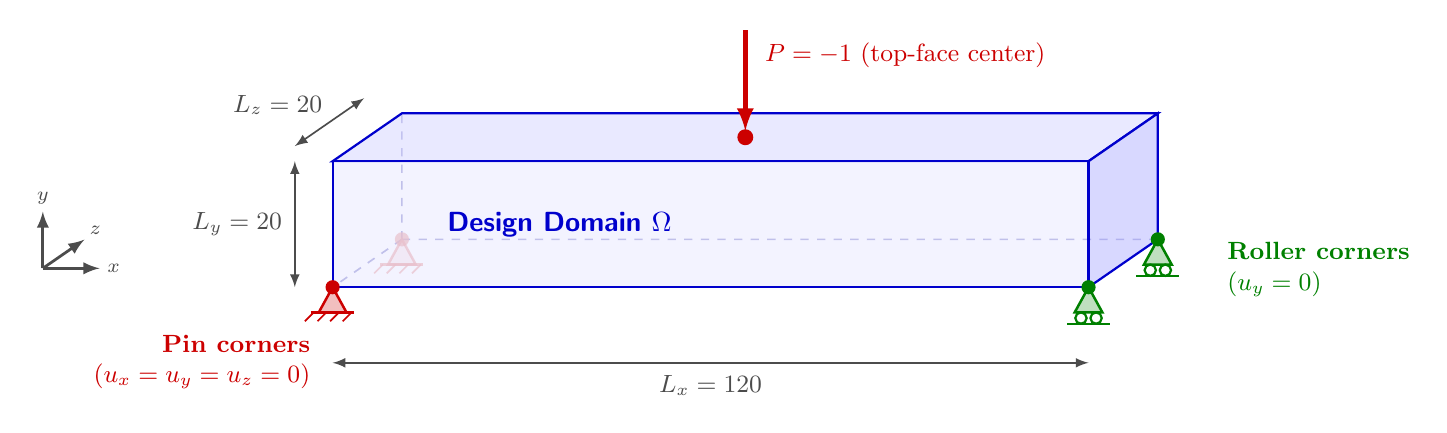
\begin{tikzpicture}[x={(1cm,0cm)}, y={(0cm,1cm)}, z={(0.55cm,0.38cm)}, scale=1.6, >=latex]
  % ============================================================
  % FullMBBBeamPoint3d: 两端底角点支承、顶面中心受集中力的完整三维 MBB 梁
  % 坐标映射与代码坐标系一致: x = 长度 (屏幕向右), y = 高度 (屏幕向上),
  % z = 宽度 (斜二测, 屏幕右上). 尺寸比例 6:1:1 对应默认 domain (0,120,0,20,0,20).
  % 可见面: 前面 z=0, 顶面 y=Ly, 右端面 x=Lx; 隐藏顶点 (0,0,Lz) 及其三条棱画虚线.
  % ============================================================
  \def\Lx{6.0}
  \def\Ly{1.0}
  \def\Lz{1.0}

  % 支座符号: 铰支 = 三角形 + 地面阴影线, 滚支 = 三角形 + 两个滚轮
  \newcommand{\pinsupport}[2]{%
    \draw[#2, line width=0.9pt, fill=#2!25] (#1) -- ++(-0.11,-0.2) -- ++(0.22,0) -- cycle;
    \draw[#2, line width=0.9pt] ($(#1)+(-0.17,-0.2)$) -- ++(0.34,0);
    \foreach \s in {-0.15,-0.05,0.05,0.15}
      \draw[#2, line width=0.6pt] ($(#1)+(\s,-0.2)$) -- ++(-0.07,-0.07);
    \fill[#2] (#1) circle (1.6pt);}
  \newcommand{\rollersupport}[2]{%
    \draw[#2, line width=0.9pt, fill=#2!25] (#1) -- ++(-0.11,-0.2) -- ++(0.22,0) -- cycle;
    \draw[#2, line width=0.8pt] ($(#1)+(-0.06,-0.245)$) circle (0.045);
    \draw[#2, line width=0.8pt] ($(#1)+(0.06,-0.245)$) circle (0.045);
    \draw[#2, line width=0.9pt] ($(#1)+(-0.17,-0.29)$) -- ++(0.34,0);
    \fill[#2] (#1) circle (1.6pt);}

  % 1. 隐藏棱 (虚线)
  \draw[blue!60!black, dashed, line width=0.6pt]
    (0,0,\Lz) -- (\Lx,0,\Lz)
    (0,0,\Lz) -- (0,\Ly,\Lz)
    (0,0,\Lz) -- (0,0,0);

  % 隐藏的左端后底角支座 (0,0,Lz), 透过前面可见
  \begin{scope}[opacity=0.7]
    \pinsupport{0,0,\Lz}{red!80!black}
  \end{scope}

  % 2. 可见面
  \draw[blue!80!black, line width=0.8pt, fill=blue!10, fill opacity=0.85]
    (0,\Ly,0) -- (\Lx,\Ly,0) -- (\Lx,\Ly,\Lz) -- (0,\Ly,\Lz) -- cycle;   % 顶面
  \draw[blue!80!black, line width=0.8pt, fill=blue!18, fill opacity=0.85]
    (\Lx,0,0) -- (\Lx,0,\Lz) -- (\Lx,\Ly,\Lz) -- (\Lx,\Ly,0) -- cycle;   % 右端面
  \draw[blue!80!black, line width=0.8pt, fill=blue!6, fill opacity=0.8]
    (0,0,0) -- (\Lx,0,0) -- (\Lx,\Ly,0) -- (0,\Ly,0) -- cycle;           % 前面

  \node[font=\sffamily\bfseries, color=blue!80!black] at (\Lx*0.3, \Ly*0.5, 0)
    {Design Domain $\Omega$};

  % 3. 可见的三个底角支座
  \pinsupport{0,0,0}{red!80!black}
  \rollersupport{\Lx,0,0}{green!50!black}
  \rollersupport{\Lx,0,\Lz}{green!50!black}

  \node[red!80!black, font=\small\bfseries, align=right, anchor=north east] at (-0.1, -0.3, 0)
    {Pin corners\\$(u_x=u_y=u_z=0)$};
  \node[green!50!black, font=\small\bfseries, align=left, anchor=west] at (\Lx+0.75, -0.05, \Lz*0.5)
    {Roller corners\\$(u_y=0)$};

  % 4. 顶面中心集中力 (x = Lx/2, y = Ly, z = Lz/2)
  \coordinate (TopCenter) at (\Lx/2, \Ly, \Lz/2);
  \draw[->, red!80!black, line width=1.8pt] ($(TopCenter)+(0,0.85,0)$) -- ($(TopCenter)+(0,0.05,0)$);
  \fill[red!80!black] (TopCenter) circle (1.8pt);
  \node[red!80!black, font=\small, anchor=west] at ($(TopCenter)+(0.08,0.65,0)$)
    {$P = -1$ (top-face center)};

  % 5. 坐标轴 (置于区域左侧, 避免与支座重叠)
  \begin{scope}[shift={(-2.3,0.15,0)}]
    \draw[->, line width=1.0pt, black!70] (0,0,0) -- (0.45,0,0) node[right=-1pt, font=\scriptsize] {$x$};
    \draw[->, line width=1.0pt, black!70] (0,0,0) -- (0,0.45,0) node[above=-1pt, font=\scriptsize] {$y$};
    \draw[->, line width=1.0pt, black!70] (0,0,0) -- (0,0,0.6)  node[above right=-2pt, font=\scriptsize] {$z$};
  \end{scope}

  % 6. 尺寸线
  \draw[<->, black!70, semithick] (0,-0.6,0) -- (\Lx,-0.6,0)
    node[midway, below=1pt, font=\small] {$L_x = 120$};
  \draw[<->, black!70, semithick] (-0.3,0,0) -- (-0.3,\Ly,0)
    node[midway, left=1pt, font=\small] {$L_y = 20$};
  \draw[<->, black!70, semithick] (-0.3,\Ly+0.12,0) -- (-0.3,\Ly+0.12,\Lz)
    node[midway, above left=-1pt, font=\small] {$L_z = 20$};
\end{tikzpicture}
\end{document}
